\chapter {Estado del Arte}
  \section {Calidad del aire en México}
    \paragraph {Los habitantes de las ciudades están expuestos a una serie de problemas ocasionadas por una mala calidad del aire. Es posible que si vives en una ciudad en  ocasiones se te irriten los ojos o la garganta, o hayas escuchado de las complicaciones que conlleva tener una cantidad elevada de contaminantes flotando en el aire.}

    \subsection{¿Cuándo se iniciaron los problemas de contaminación del aire?}
    \paragraph {Desde siempre la humanidad ha emitido contaminantes al aire, pero esto se incrementó de manera dramática a partir de la Revolución Industrial iniciada en el Reino Unido a finales del siglo XVII. En esa época, el trabajo manual fue remplazado por maquinaria, básicamente por la introducción de tecnologías que empleaban el vapor y que hacían posible tener altos niveles de producción. El problema fue que con estos avances industriales se incrementó el  uso de combustibles, tal como el petróleo y el carbón mineral, ambos indispensables para el funcionamiento de la nueva maquinaria.}

    \paragraph {Desde entonces el problema de contaminación del aire se ha convertido en una constante en muchas ciudades industriales de todo el mundo, lo que ha ocasionado problemas de salud a su población.}

    \paragraph {Algunos de los casos más dramáticos y graves son la famosa niebla tóxica londinense de 1952, el deterioro de los bosques europeos por la lluvia ácida en los años cincuenta y sesenta del siglo XX, y la grave situación de la calidad del aire en la Ciudad de México, Tokio y Sao Paulo durante las últimas décadas del siglo anterior. }

    \subsection {¿Cuáles son los contaminantes y qué efectos tienen?}
    \paragraph {Los contaminantes pueden ser emitidos de forma natural o por actividades relacionadas con el ser humano. Los fenómenos naturales que se producen en la superficie o  en el interior de la tierra –como el caso de erupciones volcánicas, que produce emisiones de gases, vapores, polvos y aerosoloes-, también contribuyen a la contaminación del aire.}
      
    \paragraph {Los principales contaminantes relacionados con la calidad del aire son el bióxido de azufre (SO2), el monóxido de carbono (CO), los óxidos  de nitrógeno (NOx), las partículas suspendidas, el plomo y el ozono.}
    
    \begin{center}
      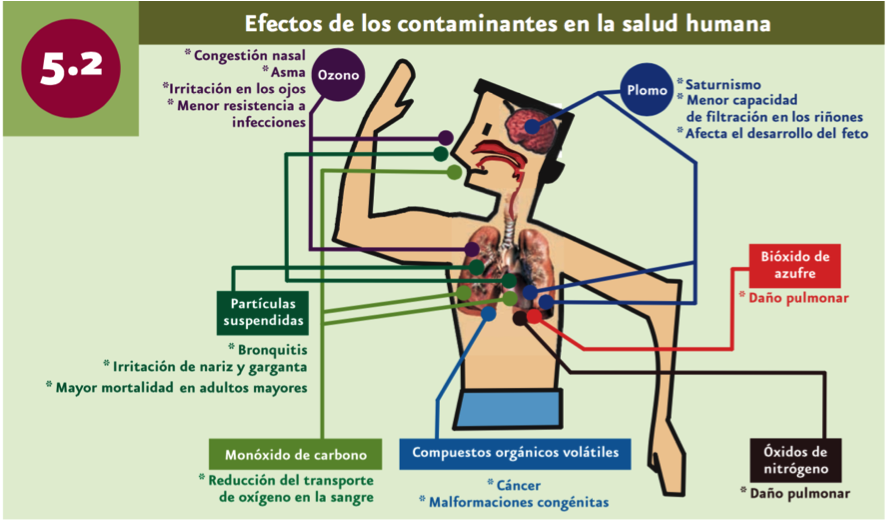
\includegraphics[width=12.5cm,height=9cm]{./images/1.png}
    \end{center}

    \paragraph {Las plantas, animales y otros organismos también resienten los efectos de contaminantes como el ozono. Principalmente con la formación de la lluvia ácida, dicha lluvia es ocasionada con la presencia de ciertos ácidos en la atomósfera que se precipitan a la tierra con la lluvia. El dióxido de azufre y los óxidos de nitrógeno, resultado de la quema de combustibles  fósiles causan lluvia ácida, ya que al combinarse con agua, oxígeno y otros compuestos químicos forman ácidos como el ácido sulfúrico y el nítrico. Las plantas se ven afectadas por esta lluvia ya que los ácidos pueden obstruir y acidificar los diminutos poros de las hojas por los que las plantas toman el aire que necesitan para realizar la fotosíntesis, además la lluvia ácida degrada los suelos, lo cual afecta las raíces y la nutrición de las plantas.}
    
    \paragraph {En el parque nacional Izta-Popo, Zoquiapan y en el Parque Nacional Desierto de los Leones, la lluvia ácida a dañado la vegetación. Estos daños involucran la pérdida de hojas y ramas, crecimiento lento y vulneravilidad a ataques de plagas y enfermedades.}
    
    \paragraph {Por otro lado los ríos, lagos y lagunas también pueden hacerse más ácidos por efecto de la lluvia ácida, lo cual pone en serio riesgo a las especies de plantas y animales que los habitan. Algunos ejemplos de estos daños se encuentran en los lagos del norte de Europa, en los que se ha reportado inclusio que han quedado sin ninguna forma de vida luego de la contaminación por lluvia ácida.}


    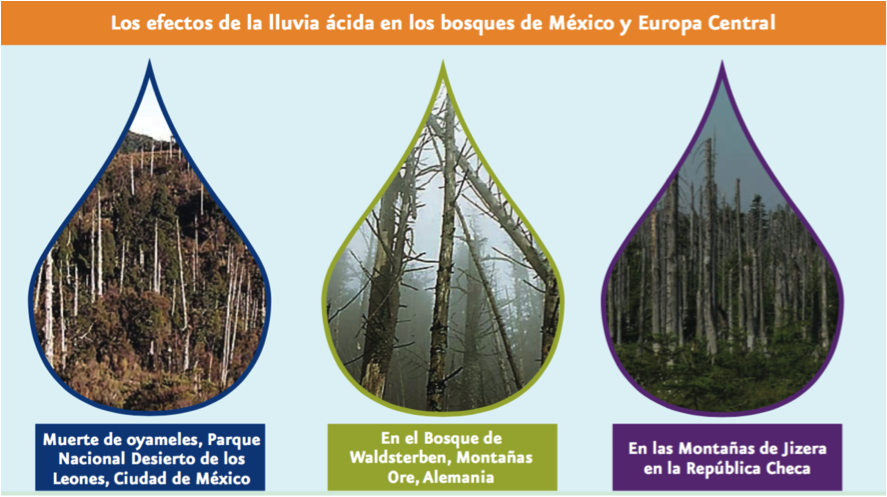
\includegraphics[width=\textwidth]{./images/2.png}
    
    \paragraph {Por otro lado también los monumentos y edificios sufren deterioros por la lluvia ácida, ya que los ácidos funcionan como agente corrosivo. El laboratorio de restauración del Instituto de Investigaciones Antropológicas de la UNAM indica que en losúltimos 25 años el deterioro de los monumentos y edificios históricos de la ciudad de México se ha acelerado de manera impresionante por el incremento de los niveles de contaminación.}

    \begin{center}
      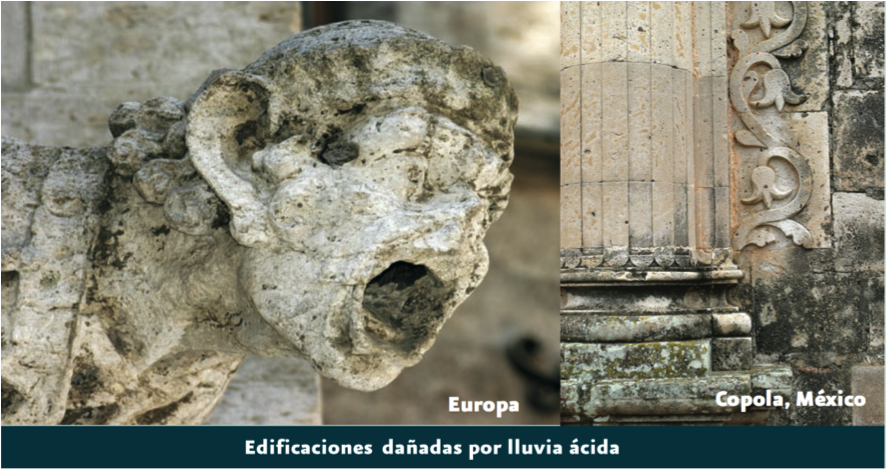
\includegraphics[width=\textwidth]{./images/3.png}
    \end{center}

    \subsection {Quiénes generan los contaminantes atmosféricos?}
    \paragraph {En México al igual que  en otros países se han desarrollado inventarios de emisiones que proporcionan información sobre la cantidad de contaminantes que se liberan al aire. En el año de 1999 de acuerdo al inventario de emisiones a nivel nacional se produjeron 40.5 millones de toneladas de las cuales el 58\ correspondieron a fuentes naturales- es decir, el suelo, la vegetación y las actividades volcánicas-    y 42\% a la contaminación de origen humano.}

    \paragraph {A pesar de que aparentemente las fuentes naturales sean las mayores productoras de contaminación, son las fuentes antropogénicas las que están cerca de la población y las que influyen en mayor medida en la calidad del aire que se respira.}

    \paragraph {Dentro de las fuentes antropogénicas, los vehículos automotores son los mayores productores de contaminantes, después la quema de gas LP y al final las emisiones de plantas generadoras de  electricidad.}

    \subsection {¿Qué hemos hecho para resolver el problema?}
    \paragraph {México lleva tiempo tomando acciones para resolver estos problemas, en 1988 implementó el Sistema Nacional del Inventario de Emisiones de Fuentes Fijas, así como un proyecto para cuantificar las emisiones del Valle de México. A partir del monitoreo de la calidad del aire ha diseñado algunas mejoras como eliminar el plomo en la gasolina, reducción del contenido de azufre.}

    \paragraph {Actualmente también existe una red de monitoreo atmosférico que abarca 52 ciudades y zonas metropolitanas que mide los niveles de contaminación presentes en el país. La concentración de los contaminantes en el aire se obtiene mediante la toma de muestras de aire que se analizan y procesan.}

    \paragraph {A partir de estas mediciones nacionales se han detectado cuales son las localidades con mayor índices de contaminación así como los contaminantes que emiten principalmente.  Uno de los esfuerzos más notables son los programas para mejorar la calidad del aire (Proaires) que buscan revertir las tendencias de deterioro, ya que incoroporan medidas para el control y abatimiento de las emisiones de los contaminantes.  También existen centrales eólicas para generar electricidad a partir de la energía del viento, una en la Venta, Oaxaca y la otra en Guerrero Negro, Baja California Sur.}

  \section {Sistemas de Monitoreo del medio Ambiente.}
    \subsection {Proyecto en la ciudad de Salamanca}
    \paragraph {Uno de los proyectos nacionales que realizo un monitoreo usando un PCFM fue realizado en la ciudad de Salamanca- una de las ciudades más contaminadas en México-.  Este proyecto es titulado “Análisis de la contaminación del aire usando un Algoritmo PCFM  aplicado a una base de datos real. La intención del estudio es analizar la relación entre contaminación y las variables ambientales. En el análisis de este estudio se involucraron datos desde Enero a Diciembre del 2007. Algunas de las variables que se incluyeron fueron S02, y la concentración de partículas menores a 10m y variables meteorológicas. Velocidad del viendo, dirección del viento, temperatura y humedad relativa. A partir de este estudio se instalaron algunos centros de monitoreo en Salamanca.}

    \subsection {Inventario Nacional de Emisiones de Gases de Efecto Invernadero (INEGEI)}
    \paragraph {En este proyecto se elabora un informe que comprende las estimaciones de las emisiones por fuente y sumidero. Esto se realiza de acuerdo a lo conforme establecido en los artículos 4 y 12 de la Convención marco de las naciones unidas sobre el cambio climático. Este proyecto es una publicación que nos ayuda a saber que deficiencias tenemos, y que efectos pudiera llegar a tener el exceso de algunos contaminantes, sin embargo no es una plataforma para accede a estos datos tan importantes.}

    \subsection {Mapa Digital -  INEGI}
    \paragraph {Este proyecto es un sistema de información geográfica que tiene como objetivo facilitar el estudio de los objetos geográficos a través del conocimiento de su ubicación espacio-temporal, así como de atributos asociados;  tales servicios bridan al usuario final la posibilidad de:}

    \begin{itemize}
      \item {Mostrar en forma gráfica la dimensión de la información contenida por medio de acercamientos, selección de capas de información, localizaciones, mediciones, etc.}
      \item {Analizar e interpretar los contenidos geográficos y estadísticos mediante operaciones matemáticas, mapas temáticos, gráficos estadísticos, análisis espacial y estadísticos básicos.}
      \item {Integrar información a través de la incorporación de datos vectoriales y raster provenientes de archivos locales, conexiones a servicios WMS y base de datos geospaciales de PostGis.}
    \end{itemize}

    \subsection {Base de Datos Estadísticos BADESNIARN}
    \paragraph {Proyecto de la SEMARNAT que presenta información integrada, revisada y validada con cada una de las fuentes. Además esta estructurada para adecuarse a las necesidades de cada usuario . El usuario en su consulta encontrará el último dato revisado con la fuente, así como la serie histórica disponible en cada caso. Finalmente la plataforma tecnológica detrás le permitirá obtener un archivo electrónica en varios formatos con la info que muestra en pantalla.}

    \paragraph { Tiene un módulo de consultas temática en donde están muy bien delimitados los temas relacionados con el ambiente, y uno dinámica en donde se asocia cada metadato o archivo con palabras clave para que el usuario pueda encontrar el tema de su interés.}

    \paragraph {
      \sloppy
      \url{http://www.semarnat.gob.mx/temas/estadisticas-ambientales/badesniar?De=SNIARN}
    }

    \subsection {Forecast IO}
    \paragraph {Es un atlas del clima que se puede visualizar a través de una página web. En el podemos consultar datos climatológicos – tales como la temperatura actual, probabilidades de precipitación - en mapas de alta definición. Este proyecto es interesante por que integra la información de diversas fuentes y también provee un servicio para obtener datos a través de peticiones REST, sin embargo estas peticiones no siempre son gratuitas.}
